% GUIDA VELOCE:
% --------------------------------------------------------------------
% X INIZIA UN UNOVO CAPITOLO:
% \chapter{??? NOME CAPITOLO}}
% \section{ ?? }
% \subsection{ ?? }
%
% --------------------------------------------------------------------
% PAROLA CONTENUTA NEL GLOSSARIO:
% scrivere la parola seguita da $^g$
% esempio: User$^g$
%
% --------------------------------------------------------------------
% PER ANDARE A CAPO SENZA RIENTRO INSERIRE:
% \\
%
% --------------------------------------------------------------------
% GRASSETO:
% \textbf{parola}
%
% --------------------------------------------------------------------
% CORSIVO:
% \emph{parola}
% --------------------------------------------------------------------
% PER SCRIVERE IN ROSSO:
% \red{parola}
%
% --------------------------------------------------------------------
% PER SCRIVERE TRA VIRGOLETTE
% ''parola''
%
% --------------------------------------------------------------------
% PER EVITARE IL RIENTRO AUTOMATICO DI UN CAPOVERSO:
% \noindent testo....
%
% --------------------------------------------------------------------

% PER SCRIVERE CARATTERI PARTICOLARI COME: { } _ ecc.. SCRIVERLI PRECEDUTI DA \
% ES: \{ \_
%
% --------------------------------------------------------------------
% X INSERIRE UN LINK:
% \url{http://www.math.unipd.it/~tullio/IS-1/2011/Progetto/C3.pdf}
%
% --------------------------------------------------------------------
% PER COMMENTARE INTERE PARTI:
% \comment{ comment }
%
% --------------------------------------------------------------------
% PER SCRIVERE NOTE DURANTE IL TESTO:
% parola \footnote{ note riguardanti la parola }
%
% --------------------------------------------------------------------
% PER SCRIVERE CODICE SORGENTE:
%
% \lstset{language=c++,
% stringstyle=\color{blue}\textrm,
% commentstyle=\rmfamily, numbers= none}

% \begin{lstlisting}
% CODICE
% \end{lstlisting}
%
% --------------------------------------------------------------------
% !!!!!!!! PER COSE + COMPLESSE VEDI: !!!!!!!!!!!!!!!!!!!!!!!
% !!!!!!!! PMAC/latex/GUIDA LATEX!!!.tex !!!!!!!!!!!!!!!!!!!!!!!

% per tutto il resto chiedi a lory prima di fare/scrivere cazzate !!!!!!!!!!



\documentclass[10pt,a4paper]{article}

\usepackage[italian]{babel}
\usepackage[T1]{fontenc}
\usepackage[utf8x]{inputenc} % uso utf8x xk x linux, mentre latin1 è per windows
\usepackage{lmodern} %insieme di font molto completo consigliato da LatexFacile pg13 in basso
\usepackage{microtype} %migliora riempimento delle righe. vedi LatexImpaziente pg41
%attiva il rientro di ogni prima riga di ogni sezione: capitolo,paragrafo ecc. vd LatexImpaziente pg41
\usepackage{indentfirst}
\usepackage{graphicx} % per inseire immagini
\usepackage[usenames,dvipsnames]{color}
\usepackage{lastpage} %serve per poter scrivere page 1 of N
% setta i bordi della pagina: dx e sx 3.2cm di rientro + nel lato di rilagatura rientra di altri 0mm
\usepackage[a4paper,top=3cm,bottom=3cm,left=3.2cm,right=3.2cm, bindingoffset=0mm]{geometry}
\usepackage{listings} % per inserire codice sorgente
\usepackage{float} % per gestire oggetti flottanti ( es immagini tabelle posizionebili con "H" che forza il posizionamento nel punto specifico )

% serve per creare tabelle lunghe + di una pagina con \begin{longtable} (vd Tabelle.pdf pg11-12)
\usepackage{longtable}

\usepackage{fancyhdr} % per impostare lo stile della pagina più personalizzato, + fancyhdr ( per regolare testatina e piè di pagina ) vedi itfancyhrd



\pagestyle{fancy}
% settaggi di pagestyle(fancy)
\lhead{
\includegraphics[scale=0.20]{images/SevenFold_small}}
%\chead{}
\rhead{\textbf{{%
\NomeDocumento - \VersioneAttuale \\ Data versione attuale: \DataRilascio \\ e-mail: \mail{sevenfold@palomino.it}}}}
\lfoot{\NomeDocumento}
\cfoot{}
\rfoot{ \textbf \thepage\ di \pageref{LastPage}}
\renewcommand{\footrulewidth}{0.4pt}

%ridefinisco il plain per cosare l'indice (a questo punto si potrebbe lasciare tutto il documento in plain
\fancypagestyle{plain}{
\lhead{
\includegraphics[scale=0.20]{images/SevenFold_small}}
%\chead{}
\rhead{\textbf{{%
\NomeDocumento - \VersioneAttuale \\ Data versione attuale: \DataRilascio \\ e-mail: \mail{sevenfold@palomino.it}}}}
\lfoot{\NomeDocumento}
\cfoot{}
\rfoot{ \textbf \thepage\ di \pageref{LastPage}}
\renewcommand{\footrulewidth}{0.4pt}
}

% da ultimo:
\usepackage{hyperref} %x l'interpretazione di indirizzi o link ipertestuali (vd LatexImpaziente pg47 )
\hypersetup{backref, colorlinks=true, linkcolor=black, urlcolor=black}

\usepackage{url} % x l'interpretazioni di internet o link ipertestuali (vd LatexImpaziente pg47 )
%\UrlFont{color =blue}
%\urlstyle{helvetic}

% Define a new 'leo' style for the package that will use a smaller font.
\makeatletter
\def\url@leostyle{%
  \@ifundefined{selectfont}{\def\UrlFont{\sf}}{\def\UrlFont{\small\ttfamily}}}
\makeatother
%% Now actually use the newly defined style.
\urlstyle{leo}


\newcommand{\mail}[1]{\textcolor{Black}{ \texttt{#1}}} %per interpretare mail (vd LatexImpaziente pg47 )
\newcommand{\cambiaFont}[2]{{\fontencoding{T1}\fontfamily{#1}\selectfont#2}}
\newcommand{\red}[1]{ \textcolor{red}{#1} } % per scrivere testo in rosso
\newcommand{\comment}[1]{} % per inserire commenti

\newcommand{\attribute}[2]{ \item[\textcolor{PineGreen}{ \texttt{#1}}] \textcolor{PineGreen}{\texttt{#2\\}}\ \ \ }
\newcommand{\method}[2]{ \item[\textcolor{MidnightBlue}{ \texttt{#1}}] \textcolor{MidnightBlue}{ \texttt{#2\\}}\ \ \ }

\newcommand{ \class}[1]{ \item[-] \texttt{#1} }
\newcommand{\virgolette}[1]{``{#1}''}



% INSERIRE QUI IL NOME DEL DOCUMENTO SEGUITO DA UNO SPAZIO
% ( così il nome si imposta in automatico nelle varie ricorrenze standard)
\newcommand{\NomeDocumento}{Scrivi in questo documento k poi uniamo tutto }

% INSERIRE QUI LA DATA DEL RILASCIO DELLA VERSIONE ATTUALE
\newcommand{\DataRilascio}{2012/04/02}

% INSERIRE LA VERSIONE ATTUALE
\newcommand{\VersioneAttuale}{v2.0.0}

% INSERIRE QUI L'ACRONIMO DEL DOCUMENTO. ESEMPIO: Analisi Dei Requisiti = AR
% Quando inserite l'acronimo qui, dovete rinominare i file presenti nella cartella
% del tipo '??-cap1-NomeCapitolo.tex' sostituendo i '??' con l'acronimo scelto!!
\newcommand{\AcronimoDocumento}{DP}

\begin{document}


% --------------------------------------------------------------------

% TITOLO ( 1° pagina)

\vspace*{2.5cm}
\begin{center}

%\cambiaFont{Cyklop}{Sevenfold}
%\cambiaFont{fve}{\Huge{Sevenfold}}

\includegraphics[scale=0.35]{images/SevenFold_big}

\vspace{2cm}

\cambiaFont{fve}{\Huge{\NomeDocumento}}\\
\vspace*{1cm}

è richiesto: circa 15 pagine a testa..

\end{center}


% --------------------------------------------------------------------

% INFORMAZIONI DEL DOCUMENTO ( 1° pagina)

\vspace*{2cm}




% --------------------------------------------------------------------

% SOMMARIO ( 2° pagina)

\newpage

\vspace*{0.5cm} % il vertical space va preceduto da una riga vuota!!!
\begin{center}

\textbf{{\huge{Sommario}}}

Questo documento contiene la struttura del sistema Woty, analizzando nel dettaglio i suoi componenti.

\vspace*{0.2cm} % il vertical space va preceduto da una riga vuota!!!

\end{center}


% --------------------------------------------------------------------



% --------------------------------------------------------------------
% INDICI:

\newpage

% INDICE CAPITOLI
\tableofcontents % genera l'indice di tutto il documento

\let\cleardoublepage\clearpage % toglie la pagina bianca dopo l'indice

% INDICE TABELLE
\listoftables

% INDICE FIGURE
\listoffigures


% --------------------------------------------------------------------

% INTRODUZIONE ( 1° CAPITOLO ) QUESTO CAPITOLO VA MESSO IN OGNI DOCUMENTO!!!!!!!!

\newpage
\section{Analisi di mercato}


%\subsection{Infortuni sul lavoro: statistiche}

\subsection{Bilanci infortunistici 2011}


\subsubsection{Visione genarale}

\url{http://www.jobtel.it/incidenti-sul-lavoro}\\

Ammontano a circa 920 i morti sul lavoro registrati nel 2011, pari a più di due persone ogni giorno.\\
Questo dato è in lieve calo rispetto ai 973 morti registrati nel 2010, ma nonostante ciò la cifra rimane ancora poco rassicurante.\\
Secondo il rapporto annuale dell'Inail anche gli infortuni sul lavoro registrati hanno visto un lieve calo, passando dai 776mila del 2010 agli 725mila del 2011, registrando una flessione del 6,6\%, pari a 51mila casi in meno.\\

\begin{figure}[H]
\centering
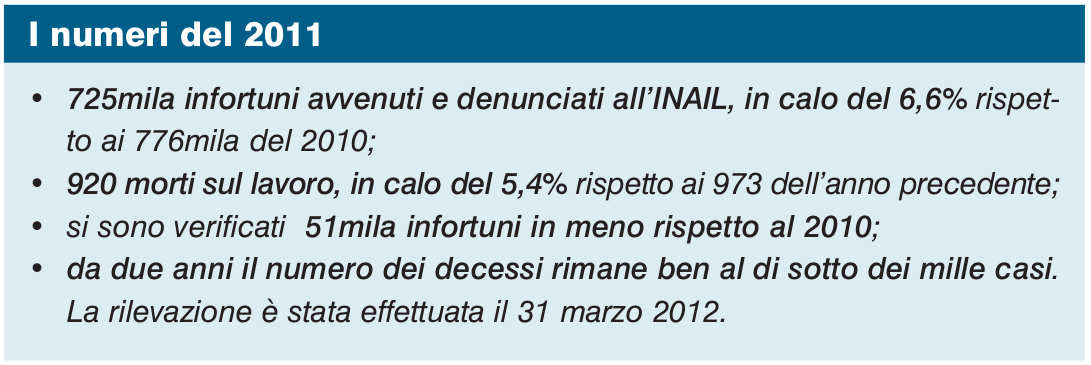
\includegraphics[scale=0.3]{images/analisiDiMercato/infortuniGenerale}
\caption{I numeri del 2011, fonti INAIL}
\end{figure}


In queste cifre non rientrano però gli infortuni relativi ai quasi 3 milioni (secondo i dati Istat) di lavoratori in nero presenti nel notro paese, tra i quali l’Istituto stima che nel 2010 (ultima proiezione disponibile) siano accaduti circa 164mila casi di infortunio.\\

\begin{figure}[H]
\centering
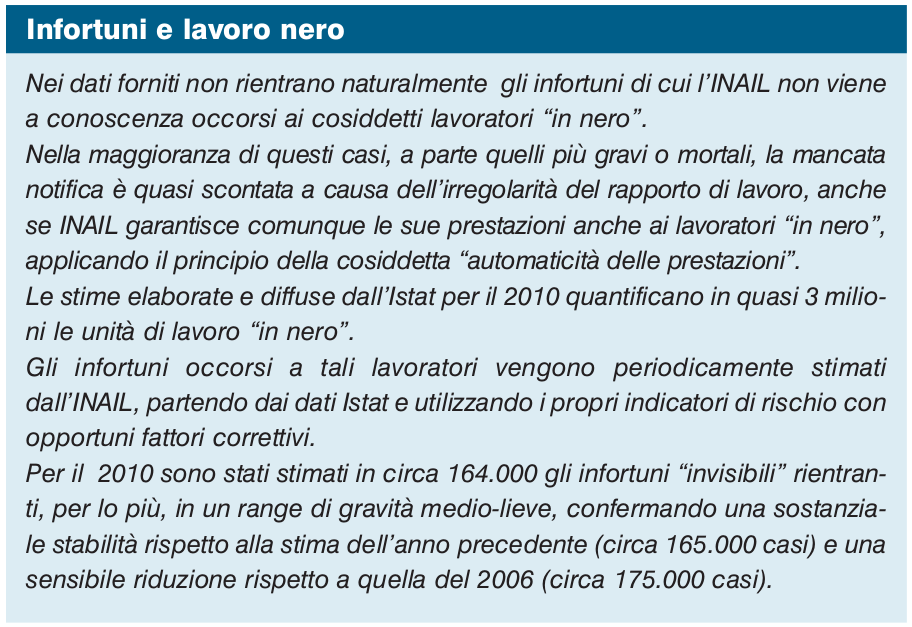
\includegraphics[scale=0.4]{images/analisiDiMercato/infortuniLavoroNero}
\caption{Infortuni e lavoro nero, fonti INAIL}
\end{figure}

Tra le 21.201 aziende controllate dall'Inail nel 2011, ben l’85,59\% è risultato ''irregolare'' per l’efficienza dei sistemi di scelta, della procedura cosiddetta di business intelligence che individua gli insiemi da controllare. Sono stati inoltre regolarizzati 48.716 lavoratori (nel 2010 erano stati 56.751), di cui 41.207 irregolari e 7.509 in nero (4.426 nel terziario, 2.675 nell’industria).\\\\



\
\
\
**business intelligence: un insieme di processi aziendali per raccogliere ed analizzare informazioni strategiche.\\\\


\subsubsection{Statistiche nel dettaglio}

Per procedere in un’analisi dettagliata dei valori sugli infortuni sul lavoro, vanno prima di tutto distinte le modalità in cui avviene l’infortunio:

\begin{itemize}
\item \textbf{in occasione di lavoro} sono i casi che avvengono nell’esercizio effettivo dell’attività;
\item \textbf{in itinere} sono invece quelli che accadono al di fuori del luogo di lavoro, durante il per-
corso casa-lavoro-casa.
\end{itemize}


E' possibile notare una diminuzione tra il 2010 e il 2011 su entrambe le tipologie di infortuni:\\
negli infortuni in itinere si è registrata una flessione del 7,1\%, passando da 88.129 casi del 2010 a 81.861 nel 2011;\\
mentre negli infortuni avvenuti in occasione di lavoro, che rappresentano circa il 90\% del com-
plesso delle denunce, la flessione è stata invece pari a 6,5\%.\\
Da notare come ben il 90\% degli infotuni si concentri unicamente nei settori lavorativi riguardanti \textit{l'industria e i servizi}: questo dato può far riflettere molto sull'utilità di sviluppare una buona prevenzione sugli infortuni sul lavoro mirata soprattutto a quensti settori fortemente a rischio.\\
Il restante 10\% degli incidenti invece è ripartito per il 6\% nel settore \textit{agricolo} e per il 4\% tra i \textit{dipendenti del conto Stato}.


\begin{figure}[H]
\centering
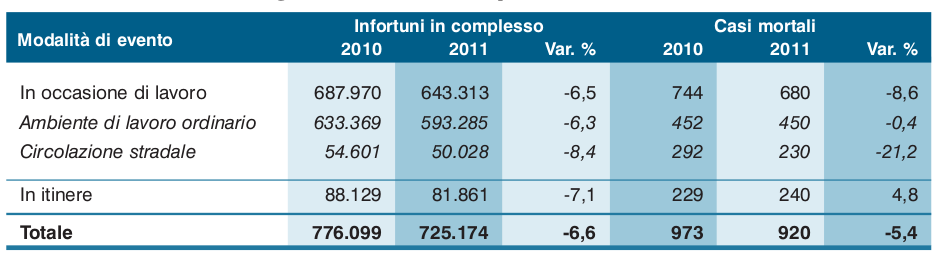
\includegraphics[scale=0.5]{images/analisiDiMercato/infortuniPerModalita}
\caption{Infortuni denunciati 2010-2011, per modalità di evento}
\end{figure}

\begin{figure}[H]
\centering
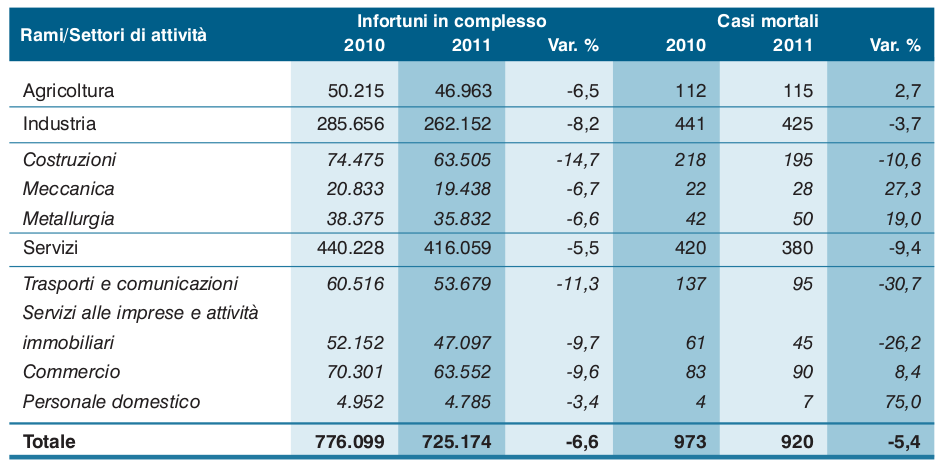
\includegraphics[scale=0.5]{images/analisiDiMercato/infortuniPerGestione2}
\caption{Infortuni denunciati 2010-2011, per gestione e settori}
\end{figure}




Nel 2011 il calo infortunistico ha interessato sia i lavoratori (-7,0\%) che le
lavoratrici (-5,6\%).\\
Per quanto riguarda invece il calo complessivo degli infortuni mortali  (-5,4\%), questa flessione è influenzata esclusivamente dei lavoratori di sesso maschile, poichè al contrario, gli infortuni mortali sul lavoro del sesso femminile, hanno riscontrato un sensibile aumento dei decessi (+15,4\%, passando dai 78 casi del 2010 ai 90 del 2011). Tale aumento è dovuto prevalentemente ai casi in itinere che rappresentano più della metà dei decessi femminili.
Per questi valori, va considerato che, secondo i dati Istat, le donne rappresentano circa il 40\% degli
occupati, e che la quota di infortuni femminili rispetto al totale è del 32\% e quasi il 10\% per
i casi mortali. Da questo \textit{si deduce che il lavoro femminile è sicuramente meno rischioso}; le donne
sono, infatti, occupate prevalentemente nei servizi e in settori a bassa pericolosità e, se
impegnate in comparti più rischiosi come quello delle Costruzioni, dei Trasporti e
dell’Industria pesante, svolgono comunque mansioni di tipo impiegatizio o dirigenziale.


\begin{figure}[H]
\centering
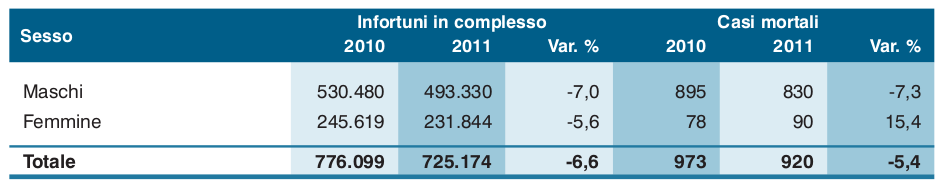
\includegraphics[scale=0.5]{images/analisiDiMercato/infortuniPerSesso1}
\caption{Infortuni denunciati 2010-2011, per sesso}
\end{figure}

\begin{figure}[H]
\centering
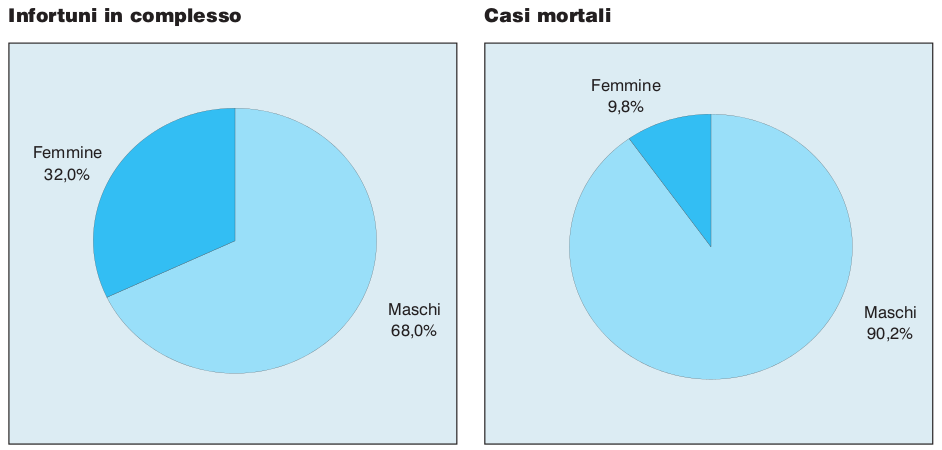
\includegraphics[scale=0.5]{images/analisiDiMercato/infortuniPerSesso2}
\caption{Infortuni per sesso, anno 2011}
\end{figure}


Analizzando i dati per fascia di età, è facile notare che la fascia tra i 35-49 risulta la più colpita con ben il 44\% di tutti gli infortuni, mentre la seconda fascia di età più colpita risulta essere quella fino ai 34 anni, con il 32\% degli infortuni complessivi.

\begin{figure}[H]
\centering
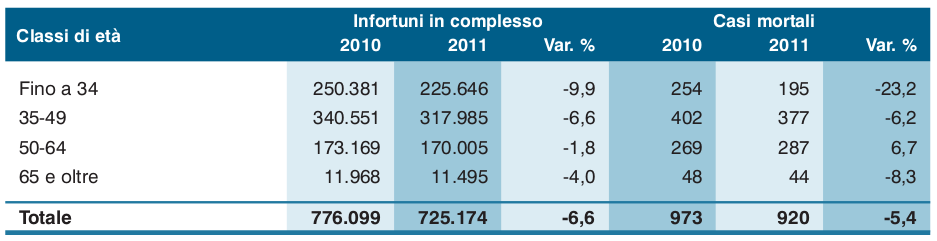
\includegraphics[scale=0.5]{images/analisiDiMercato/infortuniPerEta1}
\caption{Infortuni denunciati 2010-2011, per età}
\end{figure}

\begin{figure}[H]
\centering
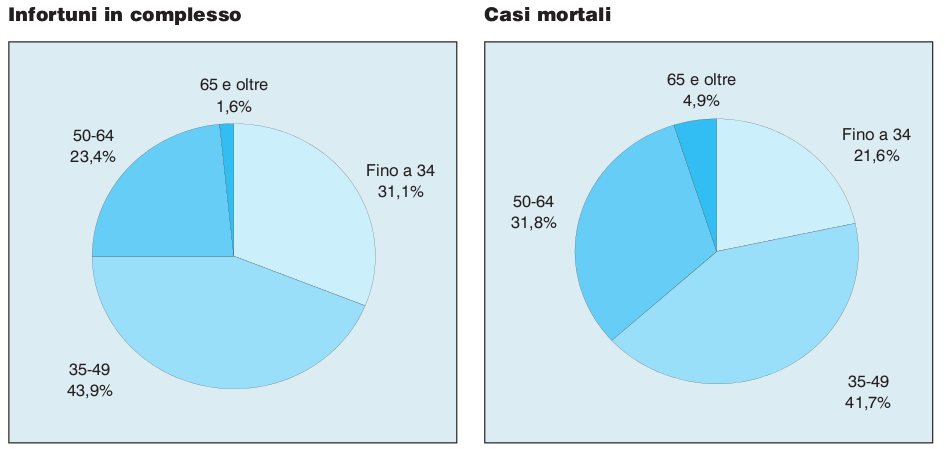
\includegraphics[scale=0.5]{images/analisiDiMercato/infortuniPerEta2}
\caption{Infortuni per età, anno 2011}
\end{figure}


\url{http://www.inail.it/Portale/appmanager/portale/desktop?_nfpb=true&_pageLabel=PAGE_SALASTAMPA&nextPage=Prodotti/Dossier_e_Speciali/SPECIALE_RAPPORTO_ANNUALE_2011/index.jsp}





conclusioni da espandere:
\begin{itemize}
\item i lavoratori + colpiti negli infortuni sono i maschi, fanno lavori + pesanti e pericolosi
\item le fascie di età + colpite sono quelle tra i 35-49 e fino ai 34 anni.
\item industria e servizi fanno il 90\% degli incidenti

\end{itemize}






\comment{
CODICE X INCLUDERE UNA IMMAGINE
(ricordati di mettere l'immagine nella cartella images!!)

\begin{figure}[H]
\centering
\includegraphics[scale=0.2]{images/XXXX}
\caption{Diagramma Gantt}
\end{figure}


}


















































\section{Concorrenza}

umba, a questo indirizzo\\\\
\url{http://www.inail.it/Portale/appmanager/portale/desktop?_nfpb=true&_pageLabel=PAGE_SALASTAMPA&nextPage=Prodotti/Dossier_e_Speciali/SPECIALE_RAPPORTO_ANNUALE_2011/index.jsp}\\\\
trovi  vari link a documenti inail sugli infortuni sul lavoro, tra cui ank questo\\\\
\url{www.inail.it/repository/ContentManagement/node/P1553662568/parte\%20TERZA\%20ricerca.pdf}\\\\
che parla di prevenzione e progetti k stanno facenso per prevenire, ti potrebbe servire per la concorrenza

\end{document}
